\section{Fibonacci chain}
\subsection{Dummy}
\begin{frame}{The Fibonacci chain}
\(
\<{7cm}{\textbf{Fibonacci numbers}}

A simple rule for generating numbers:
\begin{align*}
	F_0 &= 1 \\
	F_1 &= 1 \\
	F_2 &= F_1 + F_0 = 2 \\
	F_3 &= F_2 + F_1 = 3 \\
	F_4 &= F_3 + F_2 = 5 \\
	F_5 &= F_4 + F_3 = 8 \\
	&\vdots
\end{align*}
\[
	F_{l+2} = F_{l+1} + F_l
\]

\>

\<{7cm}{\textbf{Fibonacci words}}

Letters instead of numbers, same rule:
\begin{align*}
	C_0 &= \B \\
	C_1 &= \A \\
	C_2 &= C_1C_0 = \lett{AB} \\
	C_3 &= C_2 C_1 = \lett{ABA} \\
	C_4 &= C_3 C_2 = \lett{ABAAB} \\
	C_5 &= C_4 C_3 = \lett{ABAABABA} \\
	&\vdots
\end{align*}
\[
	C_{l+2} = C_{l+1}C_l
\]
\>
\)
\end{frame}

% counter has to be defined outside of the frame, otherwise a new counter is created at each iteration of only
\newcounter{slideno}
\begin{frame}{Fibonacci word from above}
(Infinite) Fibonacci word: \ca\cb\ca\ca\cb\ca\cb\ca\ca\cb\ca\ca\cb\dots

\ca{} $\leftrightarrow$ horizontal step, \cb{} $\leftrightarrow$ vertical step

\centering
\forloop{slideno}{1}{\value{slideno} < 14}{%
\only<\theslideno>{\includegraphics[width=.7\textwidth]{img/2_part1/CP_fibo_\theslideno}}%
}
\end{frame}

\begin{frame}{Quasiperiodicity of the Fibonacci word}
\(
\<{9cm}
\centering
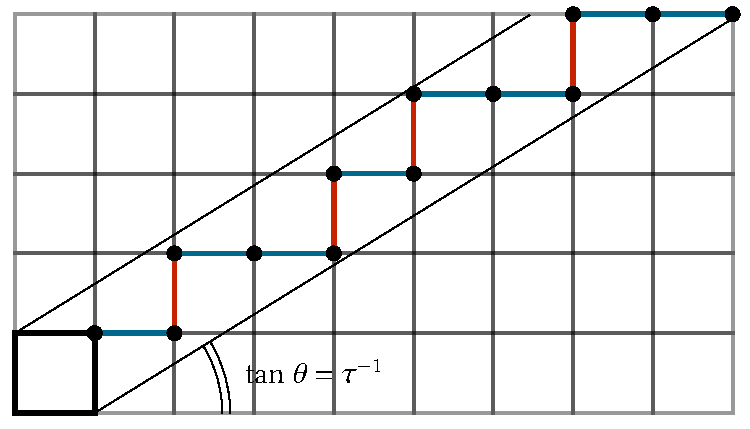
\includegraphics[width=1.\textwidth]{img/2_part1/CP_fibo_cut}
\>
\<{6cm}
\begin{itemize}
	\item average slope = inverse of the golden ratio ($\tau \simeq 1.6$)
	\item bounded fluctuations
\end{itemize}
$\to$ similar environments everywhere

$\to$ quasiperiodicity [Duneau, Katz 85]
\>
\)
\end{frame}

\begin{frame}{Cut-and-project}
\(
\<{9cm}
\centering
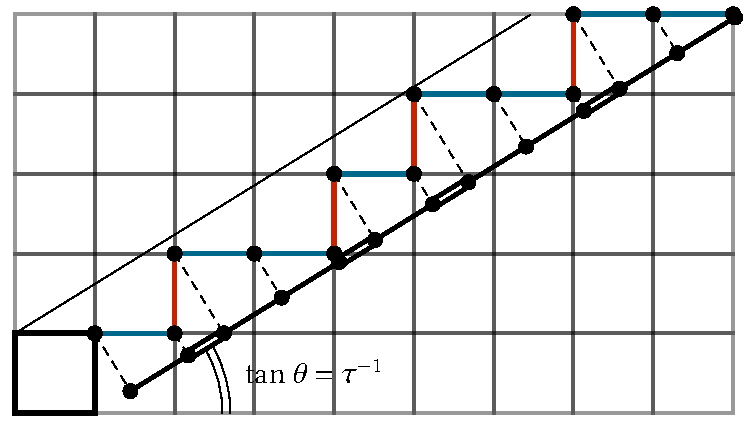
\includegraphics[width=1.\textwidth]{img/2_part1/full_cp}
\>
\<{6cm}
The cut-and-project algorithm:
\begin{enumerate}
	\item choose a hypercubic lattice (here $\zahl^2$)
	\item choose a ``physical plane'' $E_\parallel$ (here a slope)
	\item select points by translating the unit hypercube along $E_\parallel$
	\item project them onto $E_\parallel$.
\end{enumerate}
\>
\)

\textbf{\cp{} $\to$ quasiperiodic (or periodic) tiling!}
\end{frame}

\begin{frame}{From letters to atoms}
\begin{itemize}
	\item The Fibonacci word:
	\ca\cb\ca\ca\cb\ca\cb\ca\dots
	
	\item The Fibonacci (tight-binding) chain of atoms:
	
	{\centering
	%\documentclass[draft.tex]{subfiles}
%\documentclass{standalone}
%\usepackage{tikz}
%\begin{document}


    	\begin{tikzpicture}[scale=.6]
    		\newcommand{\orig}{-1.5}
    		\newcommand{\trans}{1.5}
    		\newcommand{\vertspac}{-2.}    		
    		\newcommand{\rad}{2pt} % radii of the circles
    		
    		% set the style of the strong bonds
    		\tikzset{
    			strong/.style={
    				double,
    				double distance=\rad,
    				line width=0.5pt
    				}
    		}
    	
    		% initial chain
    	
    		% bonds 
			\draw[-] (\orig+\trans,0) -- (\orig+2*\trans,0) node [midway, above] {$t_\ca$};
			\draw[strong] (\orig+2*\trans,0) -- (\orig+3*\trans,0) node [midway, above] {$t_\cb$};	
			\draw[-] (\orig+3*\trans,0) -- (\orig+4*\trans,0) node [midway, above] {$t_\ca$};
			\draw[-] (\orig+4*\trans,0) -- (\orig+5*\trans,0) node [midway, above] {$t_\ca$};
			\draw[strong] (\orig+5*\trans,0) -- (\orig+6*\trans,0) node [midway, above] {$t_\cb$};
			\draw[-] (\orig+6*\trans,0) -- (\orig+7*\trans,0) node [midway, above] {$t_\ca$};
			\draw[strong] (\orig+7*\trans,0) -- (\orig+8*\trans,0) node [midway, above] {$t_\cb$};
			\draw[-] (\orig+8*\trans,0) -- (\orig+9*\trans,0) node [midway, above] {$t_\ca$};
    	
    	
    		% sites
		    \filldraw (\orig+1*\trans,0) circle (\rad);% node [below] {6};
		    \filldraw (\orig+2*\trans,0) circle (\rad);% node [below] {3};
		    \filldraw (\orig+3*\trans,0) circle (\rad);% node [below] {8};
		    \filldraw (\orig+4*\trans,0) circle (\rad);% node [below] {5};
		    \filldraw (\orig+5*\trans,0) circle (\rad);% node [below] {2};
		    \filldraw (\orig+6*\trans,0) circle (\rad);% node [below] {7};
		    \filldraw (\orig+7*\trans,0) circle (\rad);% node [below] {4};
		    \filldraw (\orig+8*\trans,0) circle (\rad);% node [below] {1};
		    \filldraw (\orig+9*\trans,0) circle (\rad) node [right] {\dots};
		      
		\end{tikzpicture}

%\end{document}%
	}

\end{itemize}
Hamiltonian:
\[
	\op{H} = - \sum_m t_m \ket{m-1} \bra{m} + \hc
\]
Schrödinger equation for the eigenstate of energy $E$:
\[
	E \psi(m) = -t_{m}\psi(m-1) -t_{m+1}\psi(m+1)
\]
\end{frame}

\begin{frame}{The broccoli $E=0$ state}
\(
\<{6cm}
\centering
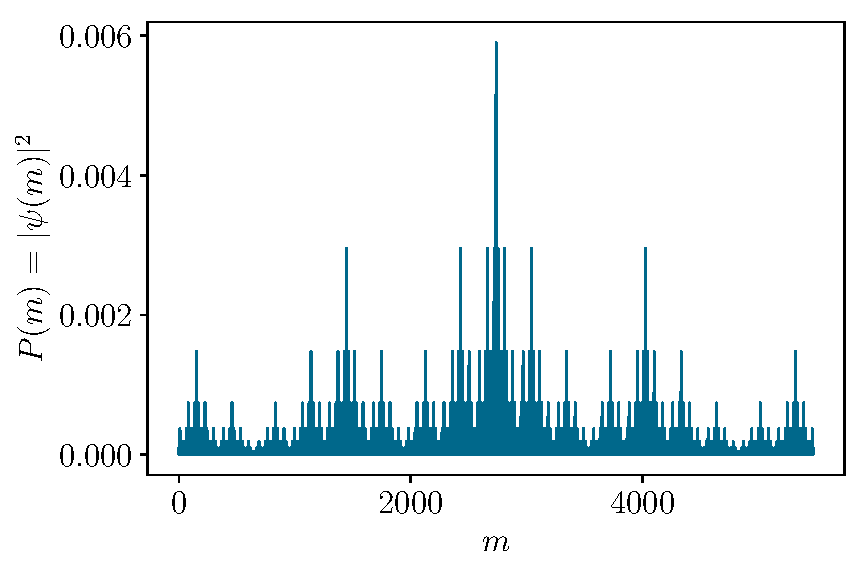
\includegraphics[width=1.\textwidth]{img/2_part1/state_fibo}

{\ss ``Romanesco broccoli'' fractal state at energy $E=0$}
\>
\<{8cm}
\begin{itemize}
	\item State at 0 energy verifies
	\[ t_m \psi(m-1) + t_{m+1}\psi(m+1) = 0 \]
	\item Fibonacci chain decouples into two chains:
	
	{\centering	
	\documentclass[../talk.tex]{subfiles}
\begin{document}


    	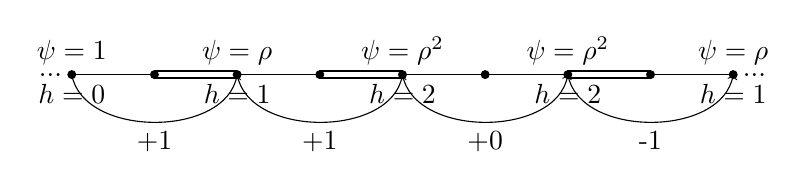
\begin{tikzpicture}[scale=.7]
    		\newcommand{\orig}{-1.5}
    		\newcommand{\trans}{1.5}
    		\newcommand{\vertspac}{-2.}
    		\newcommand{\vertsize}{0} % vertical span of the rectangles
    		\newcommand{\del}{.2}
    		\newcommand{\rad}{2pt} % radii of the circles

    		
    		% set the style of the strong bonds
    		\tikzset{
    			strong/.style={
    				double,
    				double distance=\rad,
    				line width=0.5pt
    				}
    		}
    	
    		% initial chain
    	
    		% bonds 
        	\draw[-] (\orig, 0)  node [left] {...}  -- (\orig+\trans, 0) node [midway, below] {};
			\draw[strong] (\orig+\trans,0) -- (\orig+2*\trans,0) node [midway, below] {};
			\draw[-] (\orig+2*\trans,0) -- (\orig+3*\trans,0) node [midway, below] {};	
			\draw[strong] (\orig+3*\trans,0) -- (\orig+4*\trans,0) node [midway, below] {};
			\draw[-] (\orig+4*\trans,0) -- (\orig+5*\trans,0) node [midway, below] {};
			\draw[-] (\orig+5*\trans,0) -- (\orig+6*\trans,0) node [midway, below] {};
			\draw[strong] (\orig+6*\trans,0) -- (\orig+7*\trans,0) node [midway, below] {};
			\draw[-] (\orig+7*\trans,0) -- (\orig+8*\trans,0) node [right] {...} node [midway, below] {};
    	
    		% sites
			\filldraw (\orig+0*\trans,0) circle (\rad) node [below] {$h=0$} node [above] {$\psi=1$};
			\filldraw (\orig+1*\trans,0) circle (\rad) node [below] {};
			\filldraw (\orig+2*\trans,0) circle (\rad) node [below] {$h=1$} node [above] {$\psi=\rho$};
			\filldraw (\orig+3*\trans,0) circle (\rad) node [below] {};
			\filldraw (\orig+4*\trans,0) circle (\rad) node [below] {$h=2$} node [above] {$\psi = \rho^2$};
			\filldraw (\orig+5*\trans,0) circle (\rad) node [below] {};
			\filldraw (\orig+6*\trans,0) circle (\rad) node [below] {$h=2$} node [above] {$\psi = \rho^2$};
			\filldraw (\orig+7*\trans,0) circle (\rad) node [below] {};
			\filldraw (\orig+8*\trans,0) circle (\rad) node [below] {$h=1$} node [above] {$\psi = \rho$};
			
			% arrow
			\path[->] (\orig+0*\trans,0) edge[bend right = 80] node [below] {+1} (\orig+2*\trans,0);
			\path[->] (\orig+2*\trans,0) edge[bend right = 80] node [below] {+1} (\orig+4*\trans,0);
			\path[->] (\orig+4*\trans,0) edge[bend right = 80] node [below] {+0} (\orig+6*\trans,0);
			\path[->] (\orig+6*\trans,0) edge[bend right = 80] node [below] {-1} (\orig+8*\trans,0);

		\end{tikzpicture}

\end{document}
	}

	\item Work on groups of two letters:
	\begin{itemize}
		\item \ca\cb{} $\leftrightarrow$ R
		\item \cb\ca{} $\leftrightarrow$ L
		\item \ca\ca{} $\leftrightarrow$ U
	\end{itemize}
	
\end{itemize}
\>
\)
\end{frame}

\begin{frame}{Structure of the broccoli}
\(
\<{8cm}
\begin{itemize}
	\item Effective chain
	\[
		\underbrace{\ca\cb}_{R}\underbrace{\ca\ca}_{U}\underbrace{\cb\ca}_{L}\underbrace{\cb\ca}_{L}\underbrace{\ca\cb}_{R}\underbrace{\ca\ca}_{U}\dots
	\]
	\item \textbf{Arrow function}: $A(R) = +1$, $A(L) = -1$, $A(U) = 0$.
	\item \textbf{Height function}: $h(m) = \sum_{n \leq m} A_n$
	\item Let $\rho = t_\cb/t_\ca$.
	\[
		\boxed{
		\psi(m) = (-1)^m \rho^{h(m)}
		}
	\]
\end{itemize}
\>
\<{8cm}
\centering
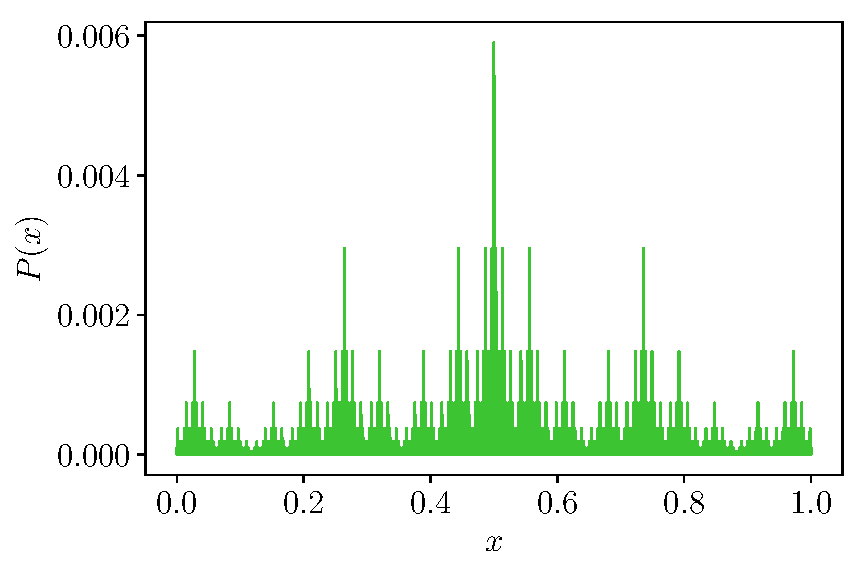
\includegraphics[width=.7\textwidth]{img/2_part1/heights_fibo}

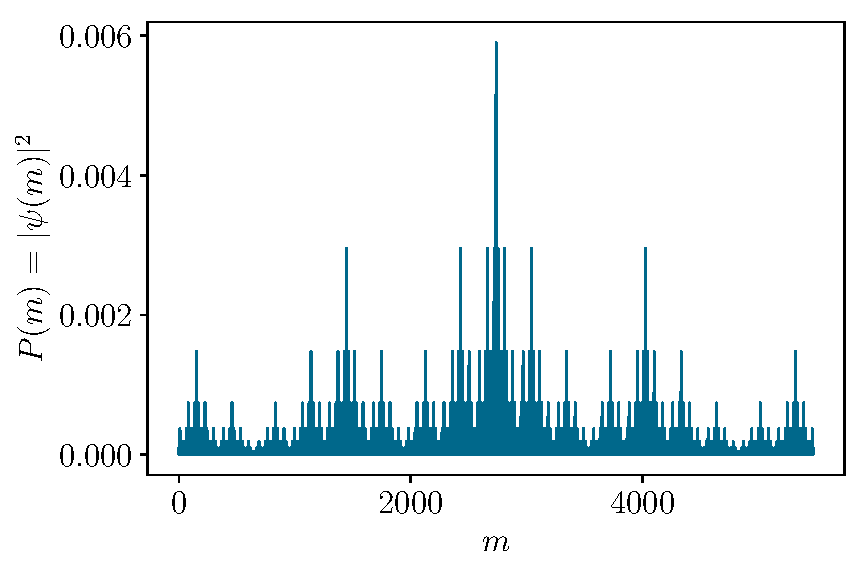
\includegraphics[width=.65\textwidth]{img/2_part1/state_fibo}
\>
\)
\end{frame}

\begin{frame}{Geometry and eigenstate properties}
\(
\<{8cm}
\begin{itemize}
	\item Arbitrary chain \ca\ca\ca\cb\cb\ca\cb\cb\dots{} (not necessarily Fibonacci)
	\item $E=0$ state: $\psi(m) = (-1)^m \rho^{h(m)}$
	\item Geometry $\leftrightarrow$ $h(m)$ function
\end{itemize}

\begin{itemize}
	\item Periodic chain: \ca\ca\ca\ca\ca\dots
%	\documentclass[../talk.tex]{subfiles}
\begin{document}

		\begin{tikzpicture}[scale=.7]
    		\newcommand{\orig}{-1.5}
    		\newcommand{\trans}{1.5}
    		\newcommand{\vertspac}{-2.}
    	
    		% initial chain
    	
    		% bonds 
        	\draw[-] (\orig+\trans,0) -- (\orig+2*\trans,0) node [midway, above] {};
			\draw[-] (\orig+2*\trans,0) -- (\orig+3*\trans,0) node [midway, above] {};	
			\draw[-] (\orig+3*\trans,0) -- (\orig+4*\trans,0) node [midway, above] {};
			\draw[-] (\orig+4*\trans,0) -- (\orig+5*\trans,0) node [midway, above] {};
			\draw[-] (\orig+5*\trans,0) -- (\orig+6*\trans,0) node [midway, above] {};
			\draw[-] (\orig+6*\trans,0) -- (\orig+7*\trans,0) node [midway, above] {};
			\draw[-] (\orig+7*\trans,0) -- (\orig+8*\trans,0) node [midway, above] {};
			\draw[-] (\orig+8*\trans,0) -- (\orig+9*\trans,0) node [midway, above] {};
			
			% wavefunction
			%\draw (\orig+4*\trans,0) -- (\orig+6*\trans,0) node [midway, above] {$\psi(r) = e^{ik r}$};
    	
    		% sites
		    \filldraw (\orig+1*\trans,0) circle (0.05) node [left] {...};
		    \filldraw (\orig+2*\trans,0) circle (0.05) node [below] {};
		    \filldraw (\orig+3*\trans,0) circle (0.05) node [below] {};
		    \filldraw (\orig+4*\trans,0) circle (0.05) node [below] {};
		    \filldraw (\orig+5*\trans,0) circle (0.05) node [below] {};
		    \filldraw (\orig+6*\trans,0) circle (0.05) node [below] {};
		    \filldraw (\orig+7*\trans,0) circle (0.05) node [below] {};
		    \filldraw (\orig+8*\trans,0) circle (0.05) node [right] {};
		    \filldraw (\orig+9*\trans,0) circle (0.05) node [right] {...};
		      
		\end{tikzpicture}
		
\end{document}
	\begin{itemize}
		\item Arrows $= 0 \implies |\psi(m)| = $ cst  
		\item \textbf{extended state}
	\end{itemize}
	\item Disordered chain: \ca\ca\ca\cb\cb\ca\cb\cb\dots
%	%\documentclass[../talk.tex]{subfiles}
%\begin{document}

\begin{tikzpicture}[scale=.7]
    		\newcommand{\orig}{-1.5}
    		\newcommand{\trans}{1.5}
    		\newcommand{\vertspac}{-2.}
    		 \newcommand{\rad}{2pt} % radii of the circles
    		 
    		% set the style of the strong bonds
    		\tikzset{
    			strong/.style={
    				double,
    				double distance=\rad,
    				line width=0.5pt
    				}
    		}
    	
    		% initial chain
    	
    		% bonds 
        	\draw[strong] (\orig+\trans,0) -- (\orig+2*\trans,0) node [midway, above] {};
			\draw[-] (\orig+2*\trans,0) -- (\orig+3*\trans,0) node [midway, above] {};	
			\draw[strong] (\orig+3*\trans,0) -- (\orig+4*\trans,0) node [midway, above] {};
			\draw[strong] (\orig+4*\trans,0) -- (\orig+5*\trans,0) node [midway, above] {};
			\draw[strong] (\orig+5*\trans,0) -- (\orig+6*\trans,0) node [midway, above] {};
			\draw[-] (\orig+6*\trans,0) -- (\orig+7*\trans,0) node [midway, above] {};
			\draw[-] (\orig+7*\trans,0) -- (\orig+8*\trans,0) node [midway, above] {};
			\draw[-] (\orig+8*\trans,0) -- (\orig+9*\trans,0) node [midway, above] {};
			
			% wavefunction
			%\draw (\orig+4*\trans,0) -- (\orig+6*\trans,0) node [midway, above] {$\psi(r) = e^{- r/\xi}$};
    	
    		% sites
		    \filldraw (\orig+1*\trans,0) circle (0.05) node [left] {...};
		    \filldraw (\orig+2*\trans,0) circle (0.05) node [below] {};
		    \filldraw (\orig+3*\trans,0) circle (0.05) node [below] {};
		    \filldraw (\orig+4*\trans,0) circle (0.05) node [below] {};
		    \filldraw (\orig+5*\trans,0) circle (0.05) node [below] {};
		    \filldraw (\orig+6*\trans,0) circle (0.05) node [below] {};
		    \filldraw (\orig+7*\trans,0) circle (0.05) node [below] {};
		    \filldraw (\orig+8*\trans,0) circle (0.05) node [right] {};
		    \filldraw (\orig+9*\trans,0) circle (0.05) node [right] {...};
		      
		\end{tikzpicture}
%\end{document}
	\begin{itemize}
		\item Random arrows $\implies |\psi(m)| \sim e^{- m^\alpha/\xi}$
		\item \textbf{localized state}
	\end{itemize}
\end{itemize}
\>
\<{8cm}
\begin{itemize}
	\item Quasiperiodic chain
	\begin{itemize}
		\item Discrete scale invariance:
	
		{\centering
		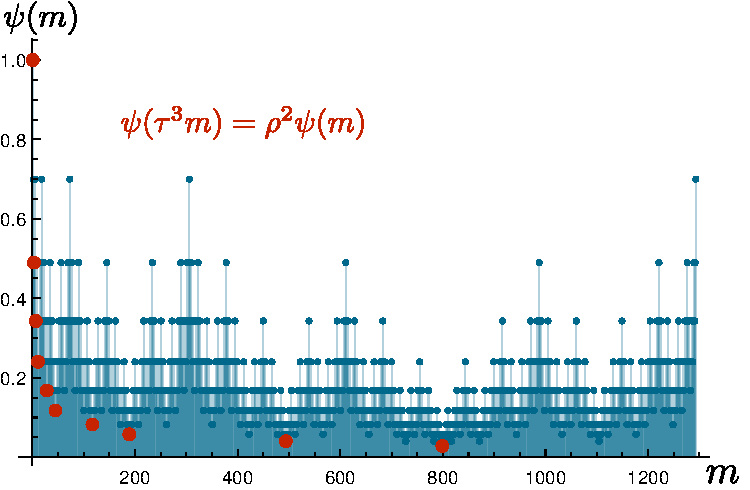
\includegraphics[width=.7\textwidth]{img/2_part1/power_law_decay}}
	
		\item Local power-law behavior $\textcolor{comp}{|\psi(m)| \sim m^{-\alpha}}$
		\item \textbf{critical state} [Kohmoto \etal{} 87]
	\end{itemize}
\end{itemize}
\>
\)
\end{frame}

\begin{frame}{Underlying scale invariance}
Fibonacci chain \emph{itself} scale invariant?

\(
\<{7cm}
\begin{itemize}
	\item Fibonacci words by concatenation:\\
	$C_2 = \lett{AB}$ \\
	$C_3 = \lett{ABA}$ \\
	$C_4 = C_3 C_2 = \lett{ABAAB}$
	
	\item Fibonacci words by \textbf{substitution}:
	\[
		\sub: 
		\begin{cases}
			\A \to \lett{AB}\\
			\B \to \A.
		\end{cases}
	\]
	$C_3 = \lett{ABA}$ \\
	$C_4 = S(C_3) = 
	\only<1>{\sub(\A)\sub(\B)\sub(\A)}
	\only<2>{\lett{AB}\sub(\B)\sub(\A)}
	\only<3>{\lett{AB}\A\sub(\A)}
	\only<4>{\lett{AB}\A\lett{AB}}
	$
\end{itemize}
\>
\<{7cm}
\begin{itemize}
	\item Infinite chain = fixed point of the substitution: \\
	$S(\lett{ABAAB}\dots) = \lett{ABAAB}\dots$
	\item Geometric substitution:
	
	{\centering
	    	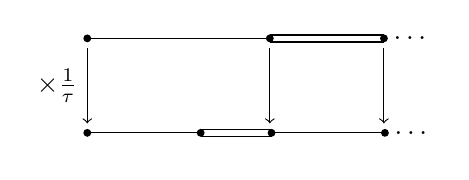
\begin{tikzpicture}[scale=.6]
    		\newcommand{\orig}{-1.5}
    		\newcommand{\s}{1.5} % length of short bonds
    		\renewcommand{\L}{2.4} % length of long bonds
    		\newcommand{\golden}{1.61}
    		\newcommand{\rs}{\golden*\s} % length of renormalized short bonds
    		\newcommand{\rL}{\golden*\L} % length of renormalized long bonds
    		\newcommand{\vertspac}{2.}    		
    		\newcommand{\rad}{2pt} % radii of the circles
    		\newcommand{\del}{0.2}
    		
    		% set the style of the strong bonds
    		\tikzset{
    			strong/.style={
    				double,
    				double distance=\rad,
    				line width=0.5pt
    				}
    		}
    	
    		%%%%%%%%%% initial chain
    		% bonds 
			\draw[-] (\orig,\vertspac) -- (\orig+\rL,\vertspac) node [midway, below] {$\A$};
			\draw[strong] (\orig+\rL,\vertspac) -- (\orig+\rs+\rL,\vertspac) node [midway, below] {$\B$};	
    		% sites
		    \filldraw (\orig,\vertspac) circle (\rad);% node [below] {6};
		    \filldraw (\orig+\rL,\vertspac) circle (\rad);% node [below] {3};
		    \filldraw (\orig+\rs+\rL,\vertspac) circle (\rad) node [right] {\dots};% node [below] {8};
		        
    		%%%%%%%%% renormalized chain
    		% bonds 
			\draw[-] (\orig,0) -- (\orig+\L,0) node [midway, below] {$\A$};
			\draw[strong] (\orig+\L,0) -- (\orig+\s+\L,0) node [midway, below] {$\B$};	
			\draw[-] (\orig+\s+\L,0) -- (\orig+\s+2*\L,0) node [midway, below] {$\A$};
%			\draw[-] (\orig+2*\s+2*\L,0) -- (\orig+2*\s+3*\L,0) node [midway, below] {$\A$};
%			\draw[strong] (\orig+2*\s+3*\L,0) -- (\orig+3*\s+3*\L,0) node [midway, below] {$\B$};
%			\draw[-] (\orig+3*\s+3*\L,0) -- (\orig+3*\s+4*\L,0) node [midway, below] {$\A$};
%			\draw[strong] (\orig+3*\s+4*\L,0) -- (\orig+4*\s+4*\L,0) node [midway, below] {$\B$};
    	
    		% sites
		    \filldraw (\orig,0) circle (\rad);% node [below] {6};
		    \filldraw (\orig+\L,0) circle (\rad);% node [below] {3};
		    \filldraw (\orig+\s+\L,0) circle (\rad);% node [below] {8};
		    \filldraw (\orig+\s+2*\L,0) circle (\rad) node [right] {\dots};% node [below] {5};
%		    \filldraw (\orig+2*\s+3*\L,0) circle (\rad);% node [below] {2};
%		    \filldraw (\orig+3*\s+3*\L,0) circle (\rad);% node [below] {7};
%		    \filldraw (\orig+3*\s+4*\L,0) circle (\rad);% node [below] {4};
%		    \filldraw (\orig+4*\s+4*\L,0) circle (\rad);% node [below] {1};

		    % arrows below rectangles
		    \draw [<-] (\orig,\del) -- (\orig,\vertspac-\del) node [midway, left] {$\times \frac{1}{\tau}$};
		    \draw [<-] (\orig+\rL,\del) -- (\orig+\rL,\vertspac-\del);
		    \draw [<-] (\orig+\rs+\rL,\del) -- (\orig+\rs+\rL,\vertspac-\del);
		      
		\end{tikzpicture}
	}
	
	\item \textbf{Infinite chain scale invariant}, scaling factor $1/\tau$.
	
\end{itemize}
\>
\)
\end{frame}

\begin{frame}{Height distribution \& multifractality}


\end{frame}

\begin{frame}{Beyond quasiperiodicity}

\end{frame}

\begin{frame}{Conclusions}

\end{frame}

\section{Renormalization group}
\subsection{Dummy}

\section{2D eigenstates}
\subsection{Dummy}